\documentclass[conference]{IEEEtran}
\IEEEoverridecommandlockouts

\usepackage[T1]{fontenc}
\usepackage[utf8]{inputenc}
\usepackage{cite}
\usepackage{amsmath,amssymb,amsfonts}
\usepackage{algorithmic}
\usepackage{graphicx}
\usepackage{textcomp}
\usepackage{xcolor}
\usepackage{booktabs}
\usepackage{array}
\usepackage{url}

\def\BibTeX{{\rm B\kern-.05em{\sc i\kern-.025em b}\kern-.08em
    T\kern-.1667em\lower.7ex\hbox{E}\kern-.125emX}}

\begin{document}

\title{A Federated Learning Approach for Layer 2 Network Intrusion Detection\\
with Explainable AI Across Distributed Network Segments}

\author{
\IEEEauthorblockN{Hosein Ghasemizade}
\IEEEauthorblockA{\textit{Department of Computer Engineering} \\
\textit{Centeral Tehran Branch}\\
Tehran, Iran\\
ghasemizade.hosein@gmail.com}
}

\maketitle

\begin{abstract}
The rapid expansion of networked environments, the proliferation of IoT devices, and
increasing reliance on cloud services have significantly broadened the attack surface of
modern networks. While existing Intrusion Detection Systems (IDS) primarily operate at
Layer~3 and above, critical attacks such as ARP Spoofing, MAC Flooding, DHCP Starvation,
and STP-based exploits occur at the Data Link Layer (Layer~2) and evade traditional
IP-based detection mechanisms. This paper proposes a federated learning framework for
Layer~2 network intrusion detection that integrates a hybrid CNN-BiLSTM deep learning
model with Explainable AI (XAI) techniques. By leveraging the FedProx aggregation
algorithm, the system addresses Non-IID data heterogeneity across distributed network
segments without transmitting raw traffic data, thereby preserving privacy. SHAP
(SHapley Additive exPlanations) is employed to interpret model decisions, enhancing
transparency and trust for security analysts. The proposed framework is evaluated against
centralized baselines across varied heterogeneity conditions, with performance measured
in terms of accuracy, F1-score, false alarm rate, communication overhead, and
computational resource consumption. The research targets practical deployment on
resource-constrained hardware and is applicable to enterprise networks, IoT
infrastructures, and edge computing environments.
\end{abstract}

\begin{IEEEkeywords}
Federated Learning, Intrusion Detection System, Layer~2 Security, Explainable AI,
SHAP, CNN-BiLSTM, FedProx, Non-IID Data, ARP Spoofing, MAC Flooding
\end{IEEEkeywords}


\section{Introduction}

The pervasiveness of computer networks and the accelerating adoption of Internet of
Things (IoT) and cloud computing have dramatically increased the attack surface that
organizations must defend. Intrusion Detection Systems (IDS) serve as a critical
component of network security infrastructure, monitoring traffic patterns to identify
anomalous behavior and potential threats~\cite{chinnasamy2025}.

Existing IDS solutions predominantly operate at the network layer (Layer~3) and above,
focusing on IP-based traffic features. This design creates a fundamental blind spot:
numerous severe attacks occur at the Data Link Layer (Layer~2) before traffic ever
reaches IP-level security controls such as firewalls. Layer~2 attacks---including ARP
Spoofing, MAC Flooding, DHCP Starvation, and Spanning Tree Protocol (STP)
manipulation---operate at the Local Area Network (LAN) infrastructure level, rarely
leaving a direct IP footprint, making them particularly difficult to detect with
conventional systems~\cite{kilincer2025,gombao2025}.

Beyond the layer-specific gap, mainstream deep learning-based IDS solutions are
predominantly centralized, requiring the transfer of raw network data to a central
server. This approach creates communication bottlenecks in large-scale distributed
networks and raises serious data privacy concerns. Furthermore, deep learning models
typically function as black boxes, limiting the ability of security analysts to
understand and verify the rationale behind detection decisions---a critical requirement
in operational security settings~\cite{belenguer2025}.

This paper addresses these three intertwined challenges by proposing a unified framework
that combines \textit{federated learning} for distributed, privacy-preserving model
training, a \textit{CNN-BiLSTM} deep learning architecture for simultaneous spatial and
temporal feature extraction, and \textit{SHAP-based Explainable AI} for model
interpretability. The remainder of this paper is organized as follows.
Section~\ref{sec:related} reviews related work. Section~\ref{sec:framework} presents
the proposed framework. Section~\ref{sec:methodology} describes the research
methodology. Section~\ref{sec:results} discusses expected results, and
Section~\ref{sec:conclusion} concludes with future directions.


\section{Related Work}
\label{sec:related}

\subsection{Intrusion Detection at the Data Link Layer}

Most IDS research has concentrated on network- and transport-layer traffic. Verkerken
et al.~\cite{verkerken2023} proposed a multi-stage hierarchical IDS that demonstrates
the benefit of layer-aware detection but still relies heavily on IP-level features for
its classification stages. Gombao~\cite{gombao2025} introduced BCAST IDS, a system
targeting broadcast-based Layer~2 anomalies, yet the approach remains centralized and
does not address privacy constraints in multi-segment deployments. Kilincer~\cite{kilincer2025}
explored an explainable AI-supported hybrid deep learning approach specifically for
Layer~2 intrusion detection, showing that SHAP-based attribution can expose meaningful
MAC-level features; however, the work assumes a single centralized training environment.
These studies collectively demonstrate both the importance and the relative immaturity
of Layer~2-focused IDS research, particularly in distributed settings.

\subsection{Federated Learning for Intrusion Detection}

Federated learning (FL) has gained considerable traction as a privacy-preserving
alternative to centralized model training. Belenguer et al.~\cite{belenguer2025}
provide a comprehensive review of FL applications in IDS, noting that the majority of
federated IDS proposals target IoT traffic or upper-layer network flows. Their survey
identifies Non-IID data distribution as the primary challenge degrading FL model
performance in heterogeneous environments and highlights FedProx as a promising
mitigation strategy. Chinnasamy et al.~\cite{chinnasamy2025} survey deep
learning-driven network IDS methods and confirm that centralized architectures dominate
the literature, with federated variants remaining comparatively underexplored.

\subsection{Explainable AI in Network Security}

Explainability is increasingly recognized as essential for operational deployment of
machine learning-based security tools. Satilmis et al.~\cite{satilmis2024} review
host-based IDS literature and note that the lack of interpretability is a consistent
barrier to adoption in enterprise environments. SHAP has emerged as a preferred
explanation technique due to its theoretical grounding in cooperative game theory and
its ability to produce both global feature importance rankings and local per-prediction
attributions. Despite this, its application within federated IDS---where explanations
must be generated locally without centralizing data---remains largely unexplored.

\subsection{Research Gap}

The survey of related work reveals that while federated IDS~\cite{belenguer2025},
Layer~2 detection~\cite{kilincer2025,gombao2025}, and XAI for security~\cite{satilmis2024}
have each been studied in isolation, no prior work simultaneously addresses all three
in the context of Data Link Layer attack detection under Non-IID conditions. This
research directly targets that gap.


\section{Proposed Framework}
\label{sec:framework}

\subsection{Framework Overview}

The proposed system is a three-tier federated architecture comprising local monitoring
agents, a federated aggregation server, and a distributed explainability module, as
illustrated conceptually in Fig.~\ref{fig:arch}. The key design principle is that raw
Layer~2 traffic never leaves its originating network segment; only model parameters
are communicated.

Figure~\ref{fig:framework} illustrates the proposed framework.

\begin{figure}[htbp]
\centering
 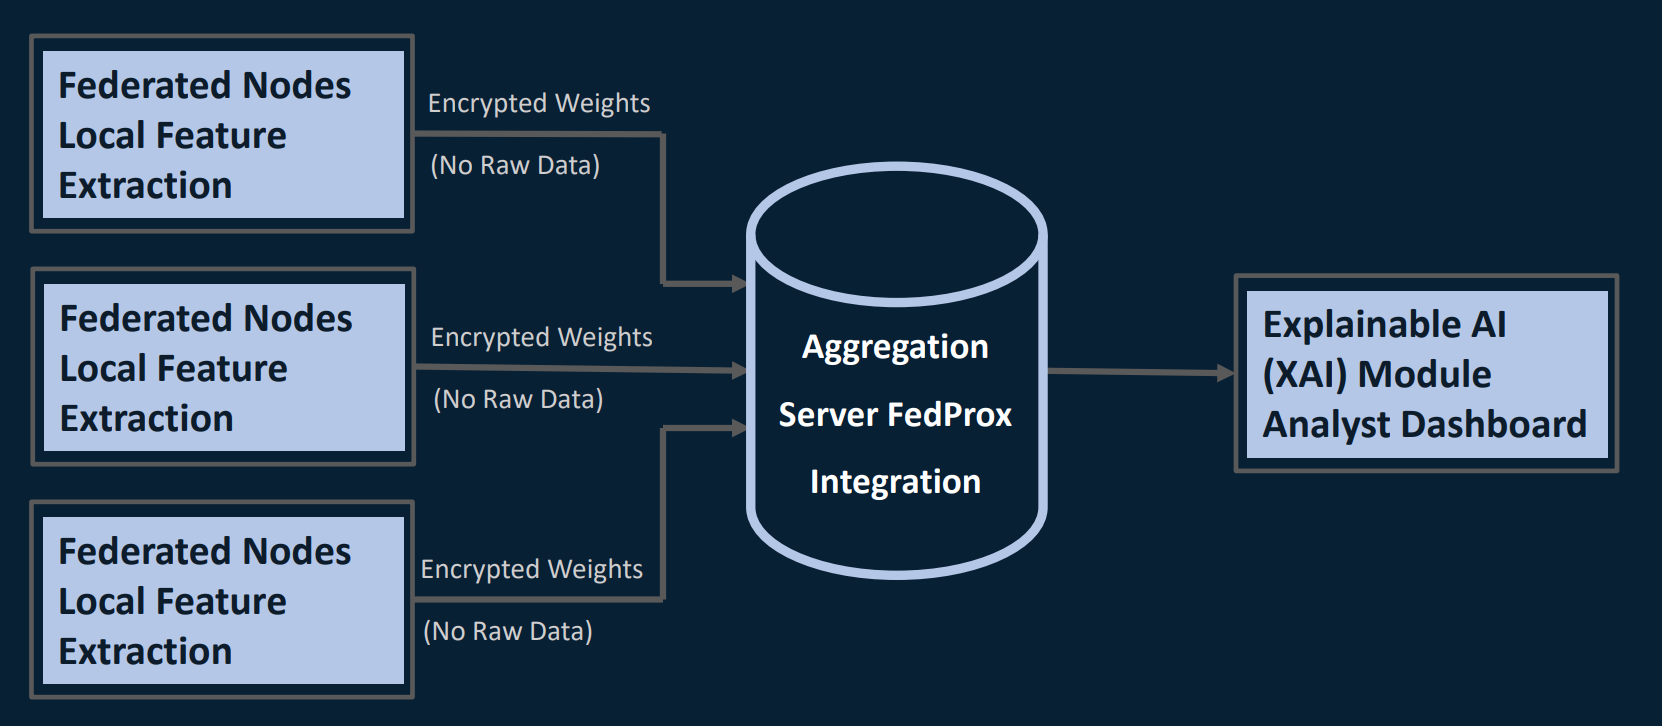
\includegraphics[width=0.45\textwidth]{framework.png}
\caption{Conceptual architecture of the proposed Federated Layer 2 IDS.}
\label{fig:framework}
\end{figure}


\subsection{Tier 1 -- Local Monitoring Agents}

Each agent is deployed at a distinct LAN segment and performs two functions: feature
extraction and local model training. At the feature extraction stage, raw Layer~2
frames are captured and transformed into structured feature vectors including MAC
address entropy, ARP request rate, broadcast-to-unicast ratio, DHCP transaction
counts, and STP Bridge Protocol Data Unit (BPDU) frequency anomalies. These features
are specifically chosen to characterize the behavioral signatures of targeted Layer~2
attacks without requiring IP-layer information.

The local model is a CNN-BiLSTM hybrid. Convolutional layers extract spatial feature
patterns within fixed-length traffic windows, while the Bidirectional LSTM layers
model temporal dependencies and sequential evolution of traffic behavior. This
combination is particularly effective for the bursty, stateful nature of Layer~2
attacks such as MAC Flooding and ARP Spoofing.

\subsection{Tier 2 -- Federated Aggregation with FedProx}

After each local training round, agents transmit only their updated model weights to
the aggregation server. The server applies the FedProx algorithm, which extends the
standard FedAvg approach by adding a proximal regularization term $\mu \| w - w^t \|^2$
to each local objective function. This term penalizes excessive deviation of local
models from the current global model, improving convergence stability when client data
distributions are heterogeneous (Non-IID). The resulting global model is redistributed
to all agents for the subsequent round.

\subsection{Tier 3 -- Distributed SHAP Explainability}

Upon global model convergence, each local agent computes SHAP values for a
representative set of detection events using its private traffic data. SHAP assigns
each feature a Shapley value quantifying its marginal contribution to a given
prediction. Security analysts can inspect these values to identify which Layer~2
features (e.g., abnormal ARP rate, MAC entropy spike) most strongly influenced a
specific alert, enabling informed triage and response without exposing raw traffic
to a central party.

\subsection{Target Attack Classes}

The framework is designed to detect the following Layer~2 attack types:
\begin{itemize}
  \item \textbf{ARP Spoofing:} Gratuitous ARP replies used to poison neighbor caches
        and enable man-in-the-middle interception.
  \item \textbf{MAC Flooding:} High-volume forged MAC address frames intended to
        exhaust switch CAM tables and force hub-mode broadcasting.
  \item \textbf{DHCP Starvation / Spoofing:} Exhaustion of the DHCP address pool or
        injection of rogue DHCP responses to redirect client traffic.
  \item \textbf{STP Manipulation:} Injection of superior BPDU frames to force
        topology changes and redirect traffic through attacker-controlled bridges.
\end{itemize}

% =================================================================
% IV. RESEARCH METHODOLOGY
% =================================================================
\section{Research Methodology}
\label{sec:methodology}

\subsection{Research Variables}

\textbf{Independent variables} are the design decisions that constitute the
experimental factors of this study, summarized in Table~\ref{tab:indvars}.

\begin{table}[htbp]
\caption{Independent Variables}
\label{tab:indvars}
\renewcommand{\arraystretch}{1.2}
\begin{tabular}{>{\bfseries}p{2.2cm} p{5.3cm}}
\toprule
Variable & Description \\
\midrule
DL Architecture    & CNN-BiLSTM vs.\ CNN-only vs.\ LSTM-only baselines \\
Training Paradigm  & Federated (FedProx, FedAvg) vs.\ centralized \\
Heterogeneity      & Non-IID degree $\alpha$ (Dirichlet distribution) \\
XAI Method         & SHAP feature attribution \\
\bottomrule
\end{tabular}
\end{table}

\textbf{Dependent variables} are the evaluation metrics used to assess system
performance, listed in Table~\ref{tab:depvars}.

\begin{table}[htbp]
\caption{Dependent Variables (Evaluation Metrics)}
\label{tab:depvars}
\renewcommand{\arraystretch}{1.2}
\begin{tabular}{>{\bfseries}p{2.2cm} p{5.3cm}}
\toprule
Metric & Description \\
\midrule
Accuracy          & Overall correct classification rate \\
Precision         & True positives among all predicted positives \\
Recall            & Fraction of actual attacks correctly detected \\
F1-Score          & Harmonic mean of precision and recall \\
False Alarm Rate  & Benign traffic incorrectly flagged as attack \\
Latency           & Per-sample inference time (ms) \\
CPU / RAM Usage   & Resource consumption during training and inference \\
Comm.\ Overhead   & Model parameter bytes exchanged per federation round \\
\bottomrule
\end{tabular}
\end{table}

\subsection{Dataset and Simulation Environment}

Experiments will be conducted using publicly available Layer~2-enriched network
traffic datasets, supplemented by traffic generated in a controlled virtual network
environment built with GNS3 and Mininet. Attack traffic will be synthesized using
Scapy and standard penetration testing tools to produce labeled ground truth for ARP
Spoofing, MAC Flooding, DHCP Starvation, and STP manipulation scenarios.

To simulate a federated environment, captured traffic will be partitioned across
virtual clients using a Dirichlet distribution with varying concentration parameter
$\alpha$ to control the degree of Non-IID heterogeneity. Low $\alpha$ values produce
highly skewed, heterogeneous distributions; high values approach IID conditions.

\subsection{Experimental Design}

The study follows a comparative experimental design with five configurations:
(1) centralized CNN-BiLSTM baseline,
(2) federated FedAvg with IID data,
(3) federated FedAvg with Non-IID data,
(4) federated FedProx with Non-IID data, and
(5) deployment of the best-performing federated model on Raspberry Pi 4 hardware
to assess resource feasibility.

Each configuration is evaluated across all dependent variables. Statistical
significance of performance differences is assessed using paired $t$-tests with
$p < 0.05$ as the significance threshold.

\subsection{Research Questions}

\textbf{Primary Question:} Can the integration of federated learning, deep learning,
and Explainable AI improve the detection of Layer~2 network attacks in distributed
settings while preserving data privacy?

\textbf{Sub-questions:}
\begin{enumerate}
  \item Can a federated Layer~2 IDS achieve detection accuracy comparable to a
        centralized counterpart?
  \item How does Non-IID data heterogeneity affect convergence, and how effectively
        does FedProx mitigate this compared to FedAvg?
  \item Which Layer~2 features are most influential in model decisions according
        to SHAP analysis?
  \item What communication and computational overhead does federated training
        introduce relative to centralized training?
  \item Is the system deployable on resource-constrained hardware while maintaining
        acceptable performance?
\end{enumerate}

% =================================================================
% V. EXPECTED RESULTS AND DISCUSSION
% =================================================================
\section{Expected Results and Discussion}
\label{sec:results}

\subsection{Detection Performance}

The CNN-BiLSTM architecture is expected to outperform single-architecture baselines
due to its dual capacity for spatial pattern recognition and temporal sequence modeling.
In centralized settings, F1-scores above 0.95 are anticipated for well-represented
attack classes such as MAC Flooding and ARP Spoofing, consistent with results reported
by Kilincer~\cite{kilincer2025} for Layer~2-focused deep learning models.

Under federated training with IID data, performance is expected to closely match the
centralized baseline, validating that the federated paradigm itself does not impose
a significant accuracy penalty when data distributions are uniform. Under Non-IID
conditions with FedAvg, a measurable degradation in convergence speed and final
accuracy is anticipated, particularly for minority attack classes. FedProx is expected
to recover a significant portion of this degradation by constraining local model drift,
consistent with findings in the federated IDS literature~\cite{belenguer2025}.

\subsection{Privacy and Communication Trade-offs}

By design, the proposed framework eliminates the transmission of raw traffic data.
Communication overhead will be quantified in terms of total parameter bytes exchanged
per global round. FedProx introduces a modest computational cost per local iteration
due to the proximal term; this is expected to be offset by faster convergence and
fewer required global rounds under Non-IID conditions.

\subsection{Explainability Insights}

SHAP analysis is expected to reveal that features related to ARP request rate and MAC
address entropy are the dominant contributors to ARP Spoofing and MAC Flooding
detections, respectively. These attributions will provide actionable guidance for
security analysts and serve as a validation mechanism for model correctness---if
SHAP highlights features that are semantically inconsistent with known attack
signatures, it would indicate spurious correlations requiring model refinement.

\subsection{Edge Deployment Feasibility}

Deployment on Raspberry Pi~4 hardware is expected to demonstrate that the local agent
component is viable on constrained devices, with inference latency remaining below
practical thresholds for near-real-time detection. Training on such devices will
require optimization (e.g., quantization or pruning) and is acknowledged as a
direction for future work.

\subsection{Broader Impact}

The results of this research will have direct implications for SOC teams, Internet
Service Providers, financial institutions, and IoT network operators. The federated,
privacy-preserving design aligns with GDPR and similar regulatory frameworks,
lowering the barrier to adoption in multi-organizational environments. The open
publication of the experimental framework and synthetic dataset generation scripts
will facilitate reproducibility and further research in this underexplored area.

% =================================================================
% VI. CONCLUSION AND FUTURE WORK
% =================================================================
\section{Conclusion and Future Work}
\label{sec:conclusion}

This paper has presented a research proposal for a federated, explainable Layer~2
network intrusion detection system. The proposal addresses three critical and
interrelated limitations of current IDS solutions: the systematic neglect of Data
Link Layer attacks, the privacy and scalability constraints of centralized deep
learning architectures, and the opacity of black-box model decision-making.

The proposed framework integrates a CNN-BiLSTM hybrid model for Layer~2 feature
extraction, FedProx-based federated aggregation to handle Non-IID data heterogeneity
across distributed network segments, and SHAP-based Explainable AI to provide
interpretable, per-prediction feature attributions to security analysts. Together,
these components form a principled and practically deployable response to each
identified limitation.

The experimental design covers centralized baselines, IID and Non-IID federated
conditions, and resource-constrained edge hardware validation, ensuring that
conclusions are both scientifically rigorous and operationally relevant.

Future work will pursue four extensions.
First, differential privacy mechanisms (e.g., Gaussian noise injection on model
gradients) will be investigated to provide formal privacy guarantees beyond the
data-locality property of federated learning.
Second, cross-domain federated scenarios---where agents represent different
organizational types such as enterprise, healthcare, and industrial IoT---will be
explored to assess generalization across heterogeneous administrative contexts.
Third, continual learning strategies will be developed to enable the global model
to adapt to emerging Layer~2 attack variants without full retraining.
Fourth, the framework will be extended to support anomaly-based detection of
zero-day Layer~2 attacks, which represent the most challenging and operationally
significant threat scenario.

% =================================================================
% REFERENCES
% =================================================================
\begin{thebibliography}{00}

\bibitem{belenguer2025}
A.~Belenguer, J.~A.~Pascual, and J.~Navaridas,
``A Review of Federated Learning Applications in Intrusion Detection Systems,''
\textit{Computer Networks}, p.~111023, 2025.

\bibitem{chinnasamy2025}
R.~Chinnasamy, M.~Subramanian, S.~V.~Easwaramoorthy, and J.~Cho,
``Deep learning-driven methods for network-based intrusion detection systems:
A systematic review,''
\textit{ICT Express}, pp.~181--215, 2025.

\bibitem{gombao2025}
J.~Gombao,
``BCAST IDS: A Novel Network Intrusion Detection,''
\textit{IEEE Access}, pp.~110289--110306, 2025.

\bibitem{kilincer2025}
I.~F.~Kilincer,
``Explainable AI supported hybrid deep learning method for layer~2 intrusion
detection,''
\textit{Egyptian Informatics Journal}, vol.~30, p.~100669, 2025.

\bibitem{satilmis2024}
H.~Satilmis, S.~Akleylek, and Z.~Yuce~Tok,
``A Systematic Literature Review on Host-Based Intrusion Detection Systems,''
\textit{IEEE Access}, vol.~12, pp.~27237--27266, 2024.

\bibitem{verkerken2023}
M.~Verkerken \textit{et al.},
``A Novel Multi-Stage Approach for Hierarchical Intrusion Detection,''
\textit{IEEE Trans.\ Netw.\ Service Manag.}, vol.~20, no.~3,
pp.~3915--3929, 2023.

\end{thebibliography}

\end{document}